%! Author = user
%! Date = 15.06.2024

\documentclass[a4paper, 14pt]{article}
%\documentclass[draft]{article}

\usepackage[T2A]{fontenc}
\usepackage[utf8]{inputenc}
\usepackage[english, russian]{babel}
\usepackage[top = 2cm, bottom = 2cm, left = 2cm, right = 2cm]{geometry}
\usepackage{indentfirst}
\usepackage{xcolor}
\usepackage{hyperref}
\usepackage{gensymb}
\usepackage{pgfplots}
\usepackage{amsmath, amsfonts, amsthm, mathtools}
\usepackage{amssymb}
\usepackage{physics, multirow, float}
\usepackage{wrapfig, tabularx}
\usepackage{icomma} % Clever comma: 0,2 - number while 0, 2 - two numbers
\usepackage{tikz, standalone}
\usepackage{fancyhdr,fancybox}
\usepackage{lastpage}
\usepackage{booktabs}
\usepackage{listings}
\usepackage{lstmisc}
\usepackage{stmaryrd}
\usepackage{amstex}

%\полуторный интервал
\onehalfspacing

\hypersetup
{   colorlinks = false,
    linkcolor = blue,
    pdftitle = {genphys},
    pdfauthor = {Володин Максим},
    allcolors = [RGB]{010 090 200}
}

\graphicspath{{./images/}}
\DeclareGraphicsExtensions{.pdf,.png,.jpg}

\restylefloat{table}
\usetikzlibrary{external}

\mathtoolsset{showonlyrefs = true} % Numbers will appear only where \eqref{} in the text LINKED
\pagestyle{fancy}

\fancyhf{}
\fancyhead[L]{Вопрос по выбору}
\fancyhead[R]{Эффект Ааронова -- Бома}
\fancyfoot[L]{}
\fancyfoot[R]{\thepage /\pageref{LastPage}}

\pgfplotsset{compat=1.18}

\begin{document}
    \begin{titlepage}
        \begin{center}
        {\large МОСКОВСКИЙ ФИЗИКО-ТЕХНИЧЕСКИЙ ИНСТИТУТ \\ \vspace{5mm}
        НАЦИОНАЛЬНЫЙ ИССЛЕДОВАТЕЛЬСКИЙ УНИВЕРСИТЕТ \\ \vspace{5mm}
        КАФЕДРА ОБЩЕЙ ФИЗИКИ}
        \end{center}
        
        \begin{center}
        {\large}
        \end{center}
        
        \vspace{5cm}
        
        {\huge
            \begin{center}
                \textbf{Вопрос по выбору}
                \\ Эффект Ааронова -- Бома
            \end{center}
        }
        
        \vspace{2cm}
        
        \begin{flushright}
        {
            Володин Максим \\
            \vspace{2mm}
            Б02-206 \\
            \vspace{2mm}
            Физтех-школа физики и исследований имени Ландау
        }
        \end{flushright}
        
        \tableofcontents \vspace{4cm}
        
        \begin{center}
            Долгопрудный \\
            17 июня 2025 года
        \end{center}
    
    \end{titlepage}
    
    \section*{Введение} \addcontentsline{toc}{section}{Введение}
    
    Реальны ли потенциал электромагнитного поля $(\varphi, A)$ или это просто математические абстракции, которые
    введены для того, чтобы было удобнее решать те или иные задачи?
    В классической физике действие силы на частицу всегда локально.
    То есть надо найти значение силы со стороны электромагнитного поля, которое действует именно в этой точке.
    И тогда сила со стороны электромагнитного поля, действующая на частицу, это есть обобщённая сила Лоренца
    
    \begin{gather}
        \vec{F} = q\left( \vec{E} + \frac{1}{c} [\vec{v}, \vec{B}] \right) \\
        \vec{E} = -\nabla \varphi - \frac{1}{c} \frac{\partial \vec{A}}{\partial t}, \quad \vec{B} =
        \operatorname{rot} \vec{A}
    \end{gather}
    
    Удобно выразить электрическое поле и $\vec{B}$, введя потенциалы $(\varphi, A)$.
    Конечно, эти потенциалы, как всякие потенциалы, неоднозначны, нужно вводить специальную калибровку, чтобы
    устранить эту неоднозначность.
    В классической физике постулируется, что реальны поля, то есть силы, а потенциалы -- это уже способ их описания
    
    В квантовой механике, где система описывается волновой функцией, оказывается возможным бессиловое влияние на
    фазу волновой функции.
    И именно это делает электропотенциалы электромагнитного поля реальными (наблюдаемыми) величинами.
    Эффект Ааронова -- Бома, авторами которого считается Аарон и Бом, хотя подобные мысли высказывались и до них
    Эренбергом и Сидаем, состоял в том, чтобы придумать такие мысленные эксперименты, которые могут, будучи
    реализованными, подтвердить физичность потенциалов поля
    
    \section*{Первый эксперимент} \addcontentsline{toc}{section}{Первый эксперимент}
    
    \begin{figure}[h]
        \centering
        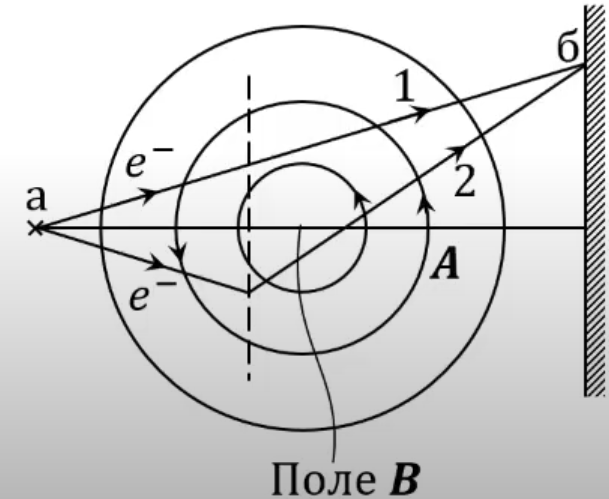
\includegraphics[width=0.4\textwidth]{exp1}
        \caption{Интерференция пучков электронов на двух щелях}
        \label{fig:exp1}
    \end{figure}
    
    Рассматриваем интерференционный опыт по типу опыта Юнга на двух щелях, схема которого дана на Рис~\ref{fig:exp1}.
    Если мы в точку А за щелями вставим бесконечно тонкий соленоид, внутри которого будет магнитное поле $\vec{B}$,
    то Ааронов и Бом показали, что результат интерференции будет сильно зависеть от векторного потенциала.
    Математически можно сказать так: если бы не было этого соленоида,(а он, грубо говоря, представляет из себя
    прокол, если вот это считать плоской картиной) и если бы прокола не было, я мог бы непрерывно деформировать путь
    этого электрона к этому электрону и разницы никакой не было.
    А проколотая плоскость не позволяет мне это сделать непрерывно.
    То есть это есть некая топологическая особенность с математической точки зрения наличия вот такого магнитного поля.
    Причем, что интересно, магнитное поле, как мы знаем, заключено внутри соленоида, снаружи его нет.
    Поэтому вдоль пути а1б и вдоль пути а2б на электрон не действуют никакие силы.
    Электрического поля нет, магнитное находится в, грубо говоря, бесконечно малой области, в соленоиде.
    Но снаружи соленоида существуют векторные линии векторного потенциала (нарисованы в виде концентрических
    окружностей)
    То есть известно, что потенциал -- векторный потенциал соленоида -- представляет из себя силовые линии и
    оказывается, что, проходя в области, где есть векторный потенциал, электрон приобретает дополнительную фазу
    волновой функции.
    А это можно продемонстрировать, сбив на экране два луча, прошедшие с разных сторон от соленоида
    
    \section*{Теоретическое описание} \addcontentsline{toc}{section}{Теоретическое описание}
    
    При наличии магнитного поля векторного потенциала вводится обобщённый импульс (большой импульс частицы не равный
    её количеству движения)
    
    \[ \vec{P} = m \vec{v} - \frac{e}{c} \vec{A} \]
    
    Посчитаем фазу (точнее, её набег) от А до Б по пути 1 и второй раз по пути А2Б.
    Тогда фаза будет зависеть формально от магнитного поля, поскольку оно тут в той или иной мере присутствует.
    
    \begin{gather}
        \Delta \varphi(B) = \frac{1}{\hbar} \int_a^b \vec{P} d \vec{l} = \frac{m}{\hbar} \int_a^b \vec{v} d \vec{l} -
        \frac{e}{c \hbar} \int_a^b \vec{A} d \vec{l} = \\
        = \Delta \varphi(0) - \frac{e}{c \hbar} \int_a^b \vec{A} d \vec{l}
    \end{gather}
    
    Это будет в единицах $\hbar$ интеграл от а до б и поскольку обобщённый импульс состоит из двух частей, то будут два
    вклада в интеграл
    
    \begin{gather}
        \Delta \varphi_1(B) = \Delta \varphi_1(0) - \frac{e}{c \hbar} \int_1 \vec{A} d \vec{l}
        \Delta \varphi_2(B) = \Delta \varphi_2(0) - \frac{e}{c \hbar} \int_2 \vec{A} d \vec{l}
    \end{gather}
    
    Первый вклад мы назовём просто фазой при нулевом магнитном поле.
    Второй же будет зависеть непосредственно от циркуляции векторного потенциала.
    Аналогично для пути а2б.
    Давайте посмотрим, с какой разностью фаз придут в точку б два электрона, которые идут разными обходящими путями
    
    \begin{gather}
        \delta(B) = \Delta \varphi_2(B) - \Delta \varphi_1(B) = \\
        = \delta(0) + \frac{e}{c \hbar}\left[\int_{a1b} \vec{A} d \vec{l} - \int_{a2b} \vec{A} d \vec{l} \right] =
        \delta(0) + \frac{e}{c \hbar} \oint \vec{A} d \vec{l} \\
    \end{gather}
    
    Здесь использована теорема Стокса, по которой интеграл был преобразован в поверхностный интеграл от
    $\operatorname{rot} \vec{A}$, и он представляет собой ничто иное, как магнитный поток через контур.
    Причем надо отметить, что магнитный поток не размазан по всему контуру, а сосредоточен только в узкой области,
    где расположен соленоид
    
    \begin{gather}
        \oint \vec{A} d \vec{l} = \int_S \operatorname{rot} \vec{A} d \vec{S} = \Phi \\
    \end{gather}
    
    Таким образом, окончательно записываем, что полная разность представляется в виде некой разности, не зависящей
    от магнитного поля, и разности фаз, зависящей от магнитного.
    
    \[ \delta(B) = \delta(0) + \frac{e}{c \hbar} \Phi = \delta(0) + 2 \pi \frac{\Phi}{\Phi_0} \]
    
    $\Phi_0$ -- это знакомый нам сверхпроводящий квант и, соответственно, сдвиг интерференционной картины напрямую
    зависит от магнитного потока, имеющегося в соленоиде
    
    \[ \Phi_0 = \frac{h c}{e} = 2 \pi \frac{\hbar c}{e} = 4,14 \cdot 10^{-7} \mathrm{Gs} \cdot \mathrm{~cm}^2 \]
    
    \section*{Экспериментальное обнаружение} \addcontentsline{toc}{section}{Экспериментальное обнаружение}
    
    \begin{figure} [h]
        \centering
        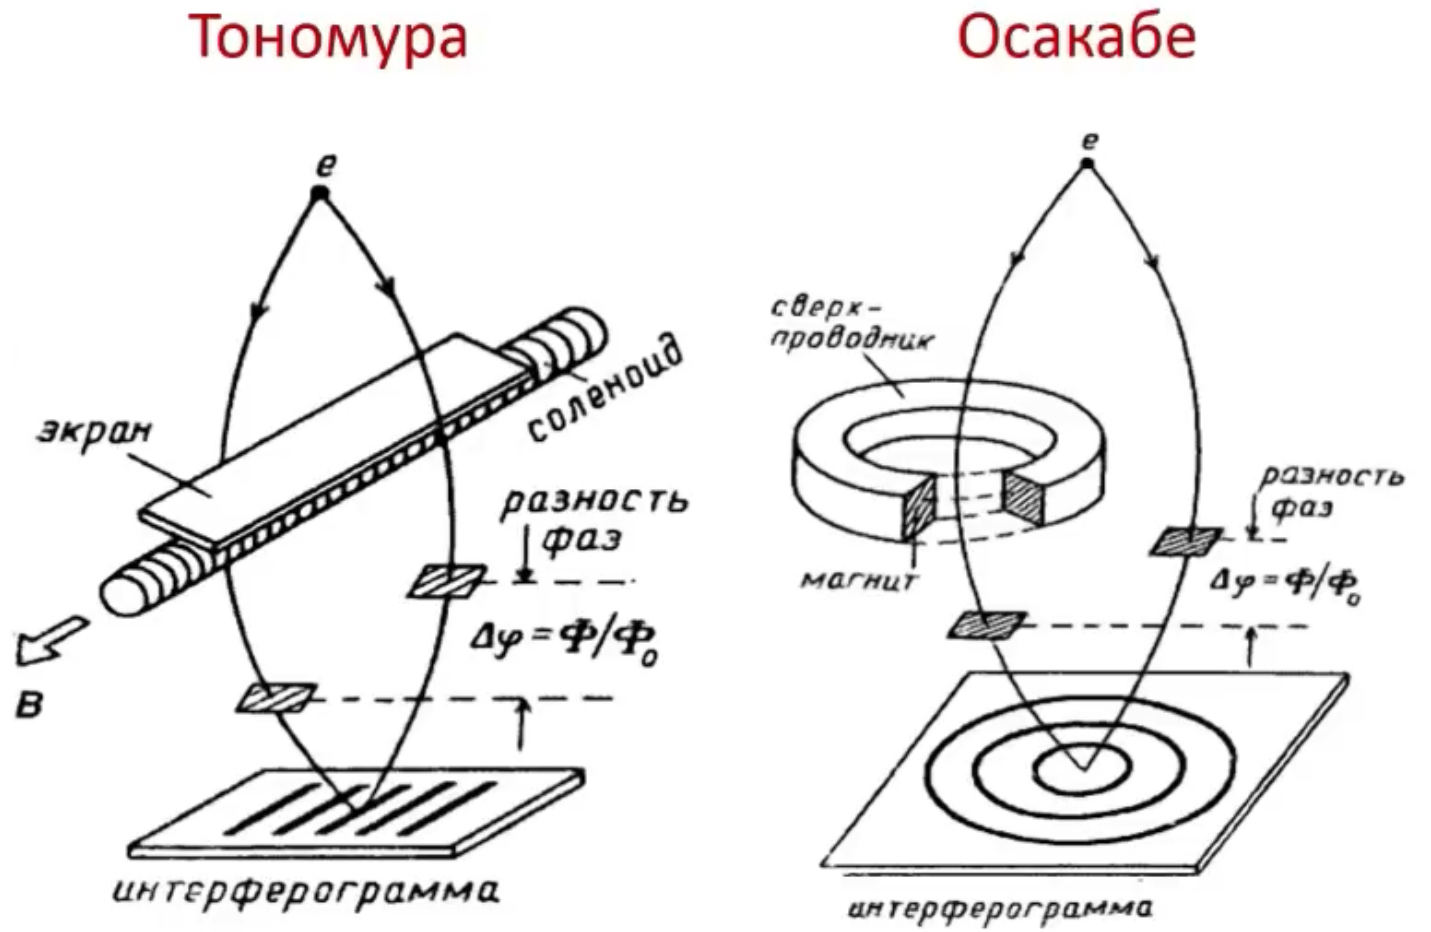
\includegraphics[width=0.8\textwidth]{exp23}
        \caption{Схемы экспериментов}
        \label{fig:exp23}
    \end{figure}
    
    Рассмотрим два эксперимента, которые были сделаны в 80-х годах на Рис~\ref{fig:exp23}.
    Первый эксперимент сделала группа физиков под руководством Тономуры.
    Идея этого опыта состояла в двухлучевой интерференции: был источник электронов; он обходил тонкий и длинный.
    Разность фаз путей на экране приводила к смещению интерференционной картины в зависимости от того, какой ток
    пропускался по соленоиду.
    Экран закрывал прямое попадание электронов.
    Тономура получил более-менее результаты, согласующиеся с формулой, но его эксперимент был подвержен критике,
    потому что не было гарантии, что все-таки силовые линии где-то там не выходят и тем не менее не оказывают действия.
    
    Окончательное и бесповоротное подтверждение положения, выдвинутое Аароновым и Бомом было сделано другим японским
    физиком Осакабе и его группой, которые воспользовались простой народной мудростью: у кольца начала нет и нет конца
    Они сделали тороидальный магнит и провели такой же опыт.
    Здесь уже, как говорится, крыть было нечем критикам: из тороидального магнита рассеяния уже никакого нет.
    
    Более того, Осакабе, как говорится, сумел убить двух зайцев: он сделал опыт два раза.
    Дело в том, что его магнит был покрыт специальной ниобиевой плёнкой, который становится сверхпроводником и поэтому
    опыт делали два раза (один раз при температуре выше критической)
    Тогда сдвиг полос согласовывался с формулой, что мы привели выше, в которой фигурирует обычный квант магнитного
    потока, не сверхпроводящий, а после охлаждения плёнки до температуры ниже критической магнитный поток внутри
    сверхпроводящей плёнки стал квантоваться.
    Это привело к тому, что части силовых линий пришлось покинуть внутренность тороидального магнита из-за
    квантования магнитного потока в сверхпроводнике и в момент фазового перехода произошёл скачок сдвига фаз и картина
    сдвинулась и соответствующий сдвиг оказался пропорционален кванту в два раза меньшему, то есть сверхпроводящему.
    Поэтому это было ещё кроме доказательства существования эффекта Ааронова -- Бома, доказательством наличия
    куперовских пар
    
    \section*{Второй эксперимент} \addcontentsline{toc}{section}{Второй эксперимент}
    
    Поскольку потенциалов было два, то Ааронов и Бом в своей работе предложили идею двухплечевого интерферометра,
    где на пути электронов были поставлены металлические трубки, на которые подавались электростатические потенциалы
    разной величины; таким образом, идея на Рис~\ref{fig:exp4} та же самая: проходя по путям ABDF и ACEF электроны
    набирали дополнительную фазу, что в конечном счёте должно было привести к сдвигу интерференционной картины, если
    бы потенциалы не подавались вообще
    
    \begin{figure}[h]
        \centering
        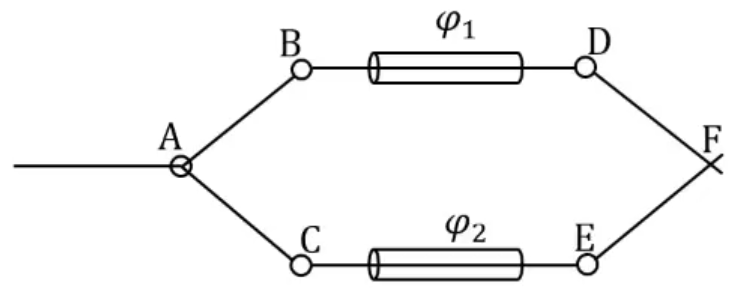
\includegraphics[width=0.8\textwidth]{exp4}
        \caption{Двухплечевой интерферометр Ааронова -- Бома}
        \label{fig:exp4}
    \end{figure}
    
    Такая же формула, только теперь интегралы по времени,которое электрон пролетает внутри трубки, в
    которой есть потенциал.
    Аналогичная формула будет для другого пути
    
    \begin{gather}
        \delta_1 = \delta(0) + \frac{e}{\hbar} \int \varphi_1 dt \\
        \delta_2 = \delta(0) + \frac{e}{\hbar} \int \varphi_2 dt \\
        \delta = \delta_2 - \delta_1
    \end{gather}
    
    К сожалению, в такой постановке сделать эксперимент не удалось, но к сегодняшнему дню получены доказательства
    для скалярного потенциала такие же надежные, как и для векторного.
    Таким образом можно считать, что в квантовой механике возможно нелокальное бессиловое воздействие на частицу.
    Раньше ещё Эйнштейн выражал бурное негодование тому, что квантовая механика допускает такие вещи
    
    \begin{thebibliography}{} \addcontentsline{toc}{section}{Список литературы}
    
        \bibitem{1} Ehrenberg, W. and R. E. Siday, «The Refractive Index in Electron Optics and the Principles of
        Dynamics», London, 8—21 (1949)
        \bibitem{2} Aharonov Y. and D. Bohm, «Significance of electromagnetic potentials in quantum theory»,
        Phys.~Rev.~115, 485—491 (1959)
        \bibitem{3} Batelaan, H. and Tonomura, A. (Sep 2009).
        The Aharonov–Bohm effects: Variations on a Subtle Theme.
        Physics Today.~62 (9): 38–43
        \bibitem{4} Osakabe, N., T. Matsuda, T. Kawasaki, J. Endo, A. Tonomura, S. Yano, and H. Yamada et al.
        Experimental confirmation of Aharonov–Bohm effect using a toroidal magnetic field confined by a superconductor
        // Physical Review A : journal.~— 1986.~— Vol.~34, №2.~ — P. 815—822
        \bibitem{5} [Источник изображений] Алексей Понятов, Эффект Ааронова—Бома.
        Наука и жизнь, 2023, № 2.~-- с.~34
    \end{thebibliography}

\end{document}